\documentclass{article}

\usepackage{polski}
\usepackage{amsmath, array}
\usepackage{graphicx}
\usepackage{float}
\usepackage{subfig}
\usepackage{multirow}
\usepackage{enumitem}
\usepackage{hyperref}
\usepackage{listings}

\NewDocumentCommand{\codeword}{v}{%
\texttt{#1}%
}

\title{Zadanie 2 - Optymalizacja LU-dekompozycji}
\author{\textbf{Łukasz Wala}\\
    \textit{AGH, Wydział Informatyki, Elektroniki i Telekomunikacji} \\
    \textit{Optymalizacja Kodu na Różne Architektury 2022/23}}
\date{Kraków, \today}


\begin{document}
\maketitle

\section{Wstęp}

Celem zadania jest zoptymalizowanie procesu LU-dekompozycji w sposób
analogiczny do laboratoriów 2, 3 oraz instrukcji dostępnych na stronie
\url{https://github.com/flame/how-to-topimize-gemm}.

Testy przeprowadzono na komputerze z procesorem Intel i3-7100 (2 rdzenie 3.9GHz).
Testy wykonywano jednowątkowo. Procesor wspiera instrukcje z rodziny SSE oraz AVX (bez AVX-512).
Użyty system operacyjny to Linux. Użyty kompilator to \codeword{gcc}.

Kod wykorzystany do testowania oraz generowania wykresów dostępny jest na końcu tego
sprawozdania.

\section{Optymalizaje}

\subsection{Kod startowy}
Rozwiązanie startowe jest inspirowane kodem LU-dekompozycji dostępnym pod adresem
\url{https://en.wikipedia.org/wiki/LU_decomposition}:

\begin{verbatim}
#define A(i, j) a[i * n + j]

/* INPUT: a - array representing matrix of size n x n
 * OUTPUT: Matrix a is changed: a=(L-E)+U such that old a=L*U.
 */
void LUDecompose(int n, double *a) {
  int i, j, k; 

  for (i = 0; i < n; i++) {
    for (j = i + 1; j < n; j++) {
      A(j, i) /= A(i, i);

      for (k = i + 1; k < n; k++)
        A(j, k) -= A(j, i) * A(i, k);
    }
  }
}
\end{verbatim}

Poniższy wykres prezentuja wydajność (\textit{GFLOPS}) wzglęzem rozmiaru macierzy (\textit{n}) dla powyższego kodu:

\begin{figure}[H]
    \centering
    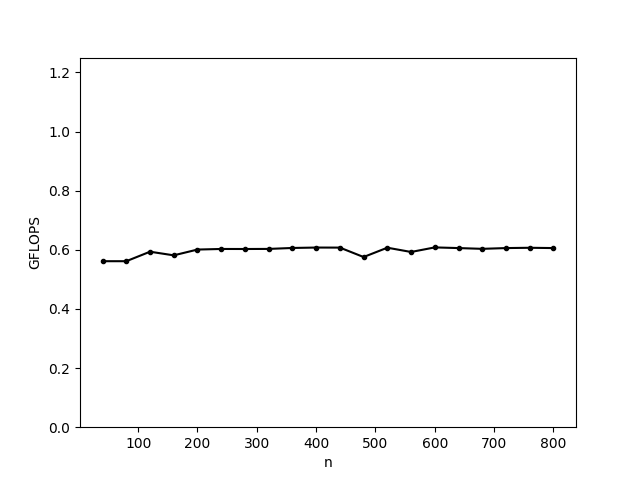
\includegraphics[width=1.0\textwidth]{figures/fig0.png}
    \caption{Przypadek bazowy}
\end{figure}

\subsection{Umieszczenie często używanych wartości w rejestrach}

Pierwszym krokiem będzie umieszczenie najczęściej używanych wartości (np. indeksów tablic)
w rejestrach.

\begin{verbatim}
#define A(i, j) a[i * n + j]

void LUDecompose(int n, double *a) {
  register int i, j, k; 
  register double div1, div2;

  for (i = 0; i < n; i++) {
    div1 = A(i, i);
    for (j = i + 1; j < n; j++) {
      A(j, i) /= div1;
      div2 = A(j, i);

      for (k = i + 1; k < n; k++)
        A(j, k) -= div2 * A(i, k);
    }
  }
}
\end{verbatim}

Te zmiany pozwalają zaobserwować znaczną poprawę w wydajności:

\begin{figure}[H]
    \centering
    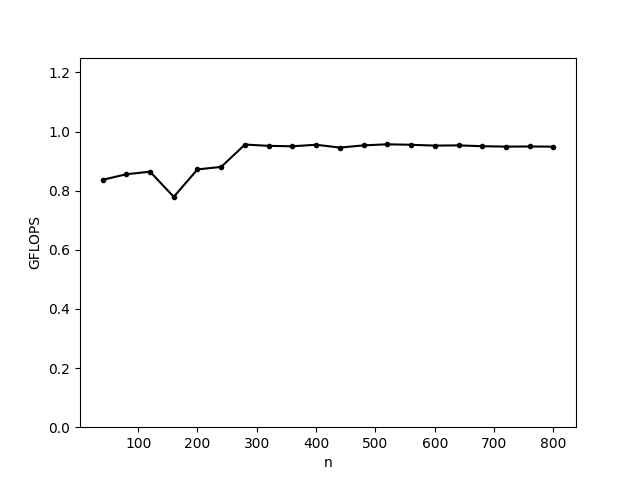
\includegraphics[width=1.0\textwidth]{figures/fig1.png}
    \caption{Po użyciu rejestrów}
\end{figure}

\subsection{Rozwinięcie pętli}

Kolejnym krokiem będzie rozwinięcie najbardziej zagnieżdżonej pętli do ośmiu iteracji.

\begin{verbatim}
#define A(i, j) a[i * n + j]
#define max(i, j) i > j ? i : j

#define BLK_SIZE 8

void LUDecompose(int n, double *a) {
  register int i, j, k; 
  register double div1, div2;

  for (i = 0; i < n; i++) {
    div1 = A(i, i);
    for (j = i + 1; j < n; j++) {
      A(j, i) /= div1;
      div2 = A(j, i);

      for (k = i + 1; k < n;)
        if (k < (max(n - BLK_SIZE, 0))) {
          A(j, k) -= div2 * A(i, k);
          A(j, k+1) -= div2 * A(i, k+1);
          A(j, k+2) -= div2 * A(i, k+2);
          A(j, k+3) -= div2 * A(i, k+3);
          A(j, k+4) -= div2 * A(i, k+4);
          A(j, k+5) -= div2 * A(i, k+5);
          A(j, k+6) -= div2 * A(i, k+6);
          A(j, k+7) -= div2 * A(i, k+7);
          k += BLK_SIZE;
        } else {
          A(j, k) -= div2 * A(i, k);
          k++;
        }
    }
  }
}
\end{verbatim}

\begin{figure}[H]
    \centering
    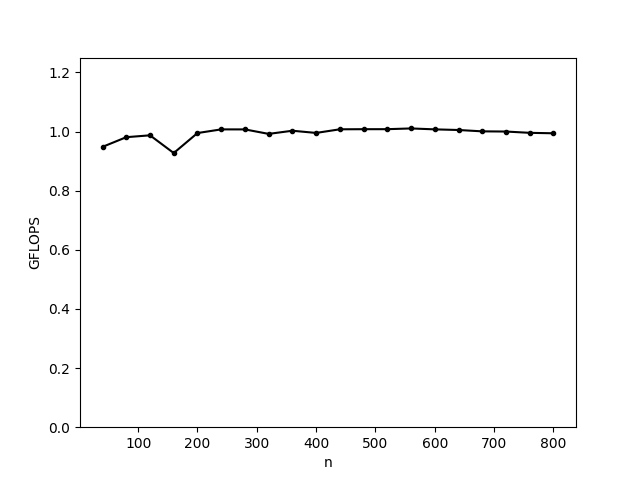
\includegraphics[width=1.0\textwidth]{figures/fig2.png}
    \caption{Po rozwinięciu pętli}
\end{figure}

Tu również występuje zauważalna poprawa wydajności

\subsection{Wprowadzenie operacji wektorowych SSE3}

Następną optymalizacją będzie użycie operacji 128-bitowych wektorowych SSE3.
Do kompilacji użyto flagi \codeword{-msse3}.

\begin{verbatim}
#include <x86intrin.h>

#define A(i, j) a[i * n + j]
#define max(i, j) i > j ? i : j

#define BLK_SIZE 8

void LUDecompose(int n, double *a) {
  register int i, j, k; 
  register double div1;
  register __m128d div2, tmp0, tmp1, tmp2, tmp3;

  for (i = 0; i < n; i++) {
    div1 = A(i, i);
    for (j = i + 1; j < n; j++) {
      A(j, i) /= div1;
      div2 = _mm_loaddup_pd(&A(j, i));

      for (k = i + 1; k < n;)
        if (k < (max(n - BLK_SIZE, 0))) {
          tmp0 = _mm_loadu_pd(&A(i, k));
          tmp1 = _mm_loadu_pd(&A(i, k+2));
          tmp2 = _mm_loadu_pd(&A(i, k+4));
          tmp3 = _mm_loadu_pd(&A(i, k+6));

          tmp0 = _mm_mul_pd(div2, tmp0);
          tmp1 = _mm_mul_pd(div2, tmp1);
          tmp2 = _mm_mul_pd(div2, tmp2);
          tmp3 = _mm_mul_pd(div2, tmp3);

          A(j, k) -= tmp0[0];
          A(j, k+1) -= tmp0[1];
          A(j, k+2) -= tmp1[0];
          A(j, k+3) -= tmp1[1];
          A(j, k+4) -= tmp2[0];
          A(j, k+5) -= tmp2[1];
          A(j, k+6) -= tmp3[0];
          A(j, k+7) -= tmp3[1];
          k += BLK_SIZE;
        } else {
          A(j, k) -= A(j, i) * A(i, k);
          k++;
        }
    }
  }
}
\end{verbatim}

\begin{figure}[H]
    \centering
    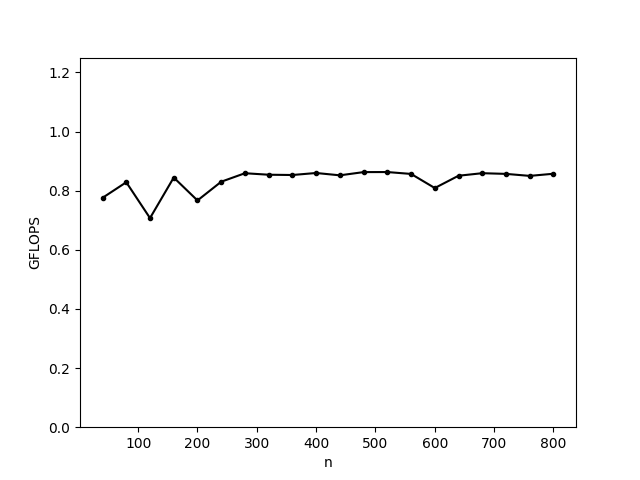
\includegraphics[width=1.0\textwidth]{figures/fig3.png}
    \caption{Po zastosowaniu instrukcji SSE3}
\end{figure}

Tutaj natomiast można zaobserwować niewielkie pogorszenie wydajności.
Powodem ku temu może być fakt, że liczba wykonywanych operacji wektorowych jest stosunkowo
niewielka względem tego, jak często wartości umieszczane są w rejestrach SSE3, czego nadkład
może być większy niż korzyści płynące z wykorzystania instrukcji wektorowych.

\subsection{Wprowadzenie operacji wektorowych AVX}

Następny krok to zastąpienie 128-bitowych operacji wektorowych SSE3 256-bitowymi operacjami AVX.
Do kompilacji użyto opcji \codeword{-mavx}.

\begin{verbatim}
#include <immintrin.h>

#define A(i, j) a[i * n + j]
#define max(i, j) i > j ? i : j

#define BLK_SIZE 8

void LUDecompose(int n, double *a) {
  register int i, j, k; 
  register double div1;
  register __m256d div2, tmp0, tmp1;
  __m128d div_tmp;

  for (i = 0; i < n; i++) {
    div1 = A(i, i);
    for (j = i + 1; j < n; j++) {
      A(j, i) /= div1;
      div_tmp = _mm_loaddup_pd(&A(j, i));
      div2 = _mm256_broadcast_pd(&div_tmp);

      for (k = i + 1; k < n;)
        if (k < (max(n - BLK_SIZE, 0))) {
          tmp0 = _mm256_loadu_pd(&A(i, k));
          tmp1 = _mm256_loadu_pd(&A(i, k+4));

          tmp0 = _mm256_mul_pd(div2, tmp0);
          tmp1 = _mm256_mul_pd(div2, tmp1);

          A(j, k) -= tmp0[0];
          A(j, k+1) -= tmp0[1];
          A(j, k+2) -= tmp0[2];
          A(j, k+3) -= tmp0[3];
          A(j, k+4) -= tmp1[0];
          A(j, k+5) -= tmp1[1];
          A(j, k+6) -= tmp1[2];
          A(j, k+7) -= tmp1[3];
          k += BLK_SIZE;
        } else {
          A(j, k) -= A(j, i) * A(i, k);
          k++;
        }
    }
  }
}
\end{verbatim}

\begin{figure}[H]
    \centering
    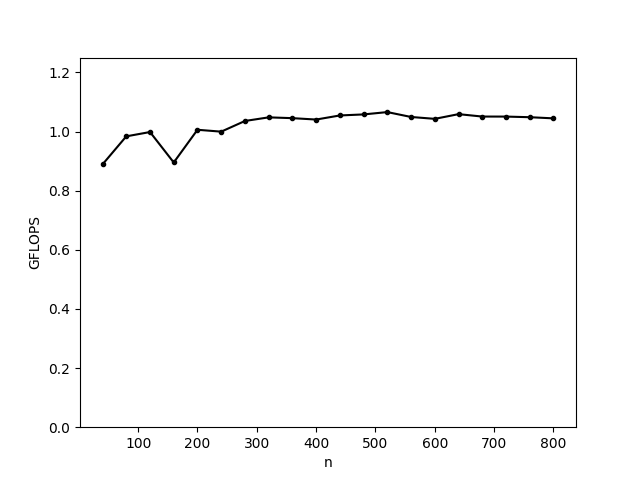
\includegraphics[width=1.0\textwidth]{figures/fig4.png}
    \caption{Po zastosowaniu instrukcji AVX}
\end{figure}

Zastosowanie 256-bitowych operacji poskutkowało poprawą, osiągając najwyższą
dotychczas wydajność.

\subsection{Użycie opcji optymalizacji kompilatora}

Ostatnia optymalizacja to użycie flag kompilatora: \codeword{-O2} oraz \codeword{-march=native}.

Dla wersji programu przed wykorzystaniem instrukcji SSE3:

\begin{figure}[H]
    \centering
    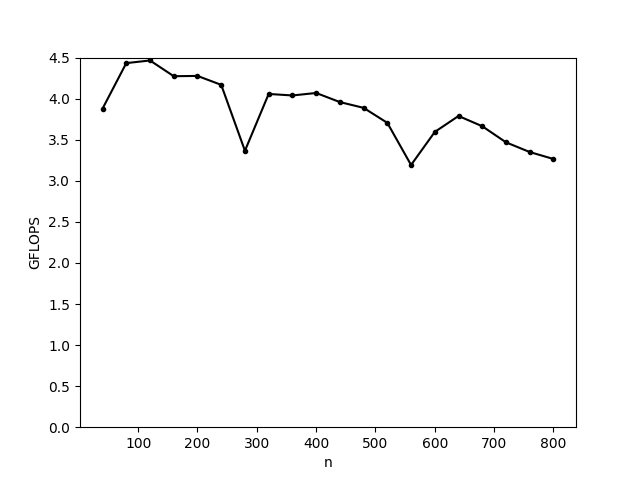
\includegraphics[width=1.0\textwidth]{figures/fig5.png}
    \caption{Z flagami kompilacji, bez instrukcji wektorowych}
\end{figure}

Dla ostatniej wersji programu, z operacjami AVX:

\begin{figure}[H]
    \centering
    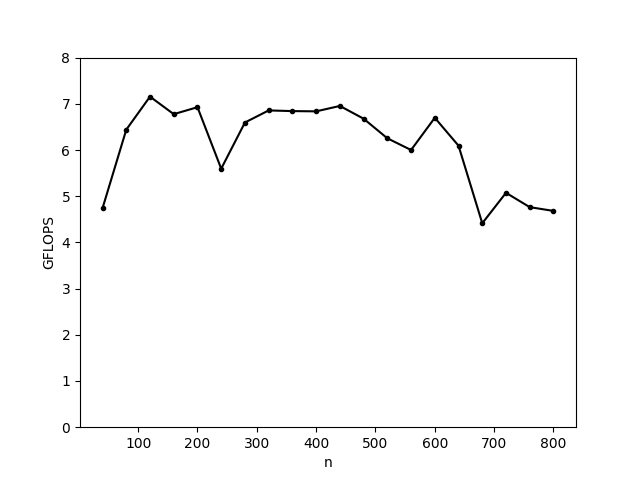
\includegraphics[width=1.0\textwidth]{figures/fig6.png}
    \caption{Z flagami kompilacji i instrukcjami wektorowymi}
\end{figure}

Użycie flag kompilacji skutkuje znaczącą poprawą, zgodnie z oczekiwaniami.

\section{Wnioski}

Powyżej przedstawione przykłady pokazują, że relatywnie niewielkim wysiłkiem można znacznie zoptymalizować
działanie dosyć prymitywnego algorytmu. Znajomosć i wykorzystanie niskopoziomowych mechanizmów, takich jak
rejestry, cache oraz dedykowane instrukcje do wykonywania obliczeń wektorowych pozwoliła na
na znacznie przyspieszenie działania programu.

\section{Kod użyty do testowania}

Testowanie rozwiązania:

\begin{verbatim}
#include <stdio.h>
#include <stdlib.h>
#include <sys/time.h>
#include <time.h>

#include "ludec4.c"

#define A(i, j) a[i * n + j]
#define B(i, j) b[i * n + j]

#define PFIRST 40 
#define PLAST 800
#define PINC 40
#define MAX_RAND 1000
#define PRINT_CHECK 0

static double gtod_ref_time_sec = 0.0;

void random_matrix(int, double*);
void copy_matrix(int, double*, double*);
double check(int, double*);
double dclock();

int main(int argc, const char *argv[]) {
  double dtime, check_val, gflops;
  double *a, *copy;
  int *p;

  for (int n=PFIRST; n<=PLAST; n+=PINC) {
    gflops = (2 * n * n * n * 1.0e-09)/3;

    a = malloc(n * n * sizeof(double));
    random_matrix(n, a);

    dtime = dclock();
    LUPDecompose(n, a);
    dtime = dclock() - dtime;

    if (PRINT_CHECK) {
      check_val = check(n, a);
      printf("N = %d, CHECK = %f\n", n, check_val);
    }

    printf("%d %f\n", n, gflops / dtime);

    free(a);
  }

  return 0;
}

double check(int n, double *a) {
  double check = 0.0;
  for (int i=0; i<n; i++) {
    for (int j=0; j<n; j++) {
      check += A(i, j);
    }
  }
  return check;
}

void random_matrix(int n, double *a) {
  srand(1);

  for (int i=0; i<n; i++) {
    for (int j=0; j<n; j++) {
      A(i, j) = rand() % MAX_RAND;
    }
  }
}

/* Adapted from the bl2_clock() routine in the BLISS library */
double dclock() {
  double the_time, norm_sec;
  struct timeval tv;

  gettimeofday(&tv, NULL);

  if (gtod_ref_time_sec == 0.0)
    gtod_ref_time_sec = (double) tv.tv_sec;

  norm_sec = (double) tv.tv_sec - gtod_ref_time_sec;

  the_time = norm_sec + tv.tv_usec * 1.0e-6;

  return the_time;
}
\end{verbatim}

Rysowanie wykresów:

\begin{verbatim}
from matplotlib import pyplot as plt

def plot_from_array(array_x, array_y):
    if len(array_x) != len(array_y):
        print("Error: length of arrays are different")
        return

    _, ax = plt.subplots()
    ax.plot(array_x, array_y, color="black", marker=".")  # marker='.'
    plt.xlabel("n")
    plt.ylabel("GFLOPS")

    plt.ylim([0, 8])

    plt.savefig("fig.png")

def results_from_file(filename):
    x = []
    y = []
    with open(filename) as file:
        lines = file.readlines()
        for line in lines:
            values = line.split() 
            x.append(int(values[0]))
            y.append(float(values[1]))

    return x, y

if __name__ == "__main__":
    x, y = results_from_file("res.txt")
    plot_from_array(x, y)
\end{verbatim}

\end{document}
